\chapter{Chromatic numbers and chromatic polynomials}

\section{Computing chromatic numbers}

The vertex, edge and total chromatic numbers can be computed using the \textit{SageMath} \cite{sagemath} function called \verb|chromatic_number| and appropriate conversions from chapter \ref{chap:clring_conversions}. Computing tables \ref{tab:platonic-chrom-nums} and \ref{tab:archimedean-chrom-nums} took less than five seconds on a computer with the Apple M2 chip.

The following two tables provide overview of vertex, edge and total chromatic numbers, denoted by $\chi(G)$, $\chi'(G)$ and $\chi''(G)$ respectively, for Platonic and Archimedean solids. Note that the edge chromatic number $\chi'(G)$ is also called the \textit{chromatic index}.

\begin{table}[H]
\centering
\begin{tabular}{l@{\hspace{1.5cm}}ccc}
\toprule
\textbf{Platonic} & \textbf{$\chi(G)$} & \textbf{$\chi'(G)$} & \textbf{$\chi''(G)$} \\
\midrule
tetrahedron & 4 & 3 & 5 \\
cube & 2 & 3 & 4 \\
octahedron & 3 & 4 & 5 \\
dodecahedron & 3 & 3 & 4 \\
icosahedron & 4 & 5 & 6 \\
\bottomrule
\end{tabular}
\caption{Vertex and edge chromatic numbers of Platonic graphs}
\label{tab:platonic-chrom-nums}
\end{table}

\begin{table}[H]
\centering
\begin{tabular}{l@{\hspace{1.5cm}}ccc}
\toprule
\textbf{Archimedean} & \textbf{$\chi(G)$} & \textbf{$\chi'(G)$} & \textbf{$\chi''(G)$} \\
\midrule
truncated tetrahedron & 3 & 3 & 4 \\
cuboctahedron & 3 & 4 & 5 \\
truncated cube & 3 & 3 & 4 \\
truncated octahedron & 2 & 3 & 4 \\
rhombicuboctahedron & 3 & 4 & 5 \\
icosidodecahedron & 3 & 4 & 5 \\
snub cube & 3 & 5 & 6 \\
truncated cuboctahedron & 2 & 3 & 4 \\
truncated icosahedron & 3 & 3 & 4 \\
truncated dodecahedron & 3 & 3 & 4 \\
rhombicosidodecahedron & 3 & 4 & 5 \\
snub dodecahedron & 4 & 5 & 6 \\
truncated icosidodecahedron & 2 & 3 & 4 \\
\bottomrule
\end{tabular}
\caption{Vertex and edge chromatic numbers of Archimedean graphs}
\label{tab:archimedean-chrom-nums}
\end{table}

Note, that from the tables above, we see that indeed all the above graphs have $\chi(G)$ at most 4. This is due to the famous \textit{Four Color Theorem} \cite{appelhaken76} for planar graphs.

Note that by using the results of the \textit{Brook's theorem} \cite{brooks41}, we have that the only graph from the table above s.t. it has $\chi(G) = \Delta(G) + 1$ should be the tetrahedron. This observation is indeed true, as we can check by consulting tables \ref{tab:platonic-basic-props} and \ref{tab:archimedean-basic-props}. 

As a consequence of \textit{Vizing's theorem} \cite{misra92}, for every graph $G$ with maximum degree $\Delta(G)$, we have $\Delta(G) \leq \chi'(G) \leq \Delta(G) + 1$. This implies two classes of graphs. Class one are graphs s.t. $\chi'(G) = \Delta(G)$. Class two are then graphs s.t. $\chi'(G) = \Delta(G) + 1$. What class are graphs of Platonic and Archimedean solids?

Let us compare the degrees at each vertex of the solids as shown in tables \ref{tab:platonic-basic-props} and \ref{tab:archimedean-basic-props} with their calculated chromatic indices in the tables above. We can observe, that all the solids are of Vizing class one. Note that this is not the case for all planar graphs. In fact, there exist planar graphs with $\Delta(G)$ from 2 up to 5 such that they are class two.

Similarly, for total coloring, Vizing's conjecture \cite{vizing68} states, that for all graphs, we have $\Delta(G) + 1 \leq \chi''(G) \leq \Delta(G) + 2$. If the conjecture holds, then it again implies two classes of graphs. In the case of Platonic and Archimedean solids, it turns out, that all of them except the tetrahedron belong to class with $\chi''(G) = \Delta(G) + 1$.

\section{Computing chromatic polynomials}


Chromatic polynomial of any graph $G=(V,E)$ can be calculated recursively using the following fact: When we fix two vertices $u$, $v$ s.t. $\{u,v\} \notin E$, we can split all colorings of $G$ into two disjoint groups. Let $d$ be the number of colorings of $G$ in which $u$ and $v$ are colored by different color and let $s$ be the number of colorings in which $u$ and $v$ are colored by same colors. Then the number of all colorings $P(G,x) = d + s$. Let $G+\{u,v\}$ be graph $G$ s.t. its set of edges is $E \cup \{u,v\}$. Let $G \cdot \{u,v\}$ be the graph $G + \{u,v\}$ where the edge $\{u,v\}$ is contracted into a single vertex. Then we can see that $d = P(G + \{u,v\},x)$ and $s = P(G \cdot \{u,v\},x)$. This fact yields the following formula \cite{chartrand2019}:
\begin{equation}\label{eqn:chrom_poly_nonedge}
 P(G,x) = P(G + \{u,v\},x) + P(G \cdot \{u,v\},x)
\end{equation}

The formula above serves as the recursive case of our computation i.e. when the graph has some non-edge. In the other case, the base case, the graph has no non-edges and thus it is a complete graph $K_n$ for some $n \in \mathbb{N}$. Then the chromatic polynomial is $P(K_n,x) = x \cdot (x-1) \cdot \ldots \cdot (x-n+1)$.

Consider this example: Given the graph of tetrahedron $K_4$ and $X$ the family of proper vertex colorings. The chromatic polynomial $P_{X}(K_4,x) = x \cdot (x-1) \cdot (x-2) \cdot (x-3)$. This can be seen if we label the vertices $v_1,v_2,v_3,v_4$ and imagine coloring them sequentially in the order of their labels. We have exactly $x$ colors left to use for the first vertex. With each other vertex, we have one less color available to use. 

\subsection{Chromatic polynomial of complete k-partite graphs with partition size 2}

In the following, let $\oplus$ denote the edge addition operation and let $\star$ denote the vertex identification operation. Let $G_{\oplus,\bar{e}}$ and $G_{\star,\bar{e}}$ describe the resulting graphs by applying the corresponding operation on some non-edge $\bar{e}$ of $G$. Let $\bar{E}$ denote the set of all non-edges of $G$.
\begin{defn}[set of non-edges]
    Let $G=(V,E)$ be a graph. We denote $\bar{E} = \bar{E}(G) = \binom{V}{2} \setminus E$ the set of non-edges of $G$.
\end{defn}

\begin{defn}[vertex identification operation]
    For a graph $G=(V,E)$ and a non-edge $\{u,v\}$ we define the resulting graph $G_{\star,\{u,v\}} = (V',E')$ as follows:
    \begin{enumerate}
        \item $V' := (V \setminus \{u,v\}) \cup \{w\}$
        \item $E' = (\binom{V'}{2} \cap E) \cup \{\{w,x\} : \{u,x\} \in E \vee \{v,x\} \in E\}$
    \end{enumerate}
    In the above, we assume that $w \notin V$.
\end{defn}

Notice, for each $\bar{e} = \{u,v\}\in \bar{E}(G)$ it holds that $|\bar{E}(G_{\star,\bar{e}})| < |\bar{E}(G)|$. This is because $\{u,v\} \notin \bar{E}(G_{\star,\bar{e}})$ and also for the new vertex $w$, we have: \[\{w,x\} \in \bar{E}(G_{\star,\bar{e}}) \implies \{u,x\} \in \bar{E}(G) \wedge \{v,x\} \in \bar{E}(G)\]
In other words, the number of non-edges after $\star$ operation always decreases.

\begin{lemma}
\label{lemma:non-edge_set_size}
    Let $G = K_{k \times (<n)}$ be a complete $k$-partite graph where each independent set has size at most $n$. Then for any non-edge $\bar{e} \in \bar{E}(G)$ and $o \in \{\oplus,\star\}$ we have that: \[|\bar{E}(G_{o,\bar{e}})| = |\bar{E}(G)| - 1\]
\end{lemma}

\begin{proof}
    Let us consider any $\bar{e} \in \bar{E}$. The operation $\oplus$ removes $\bar{e}$ from $\bar{E}$ and keeps the other non-edges intact, so the lemma holds for this case. For the case of $\star$ operation, $\bar{E}(G_{\star,\bar{e}})$ will no longer contain the non-edge $\bar{e}=\{v,u\}$. Also, since the graph is complete $k$-partite, there exists no $w \in V(G) \setminus \{v,u\}$ s.t. $\{w,v\} \in \bar{E}$ or $\{w,u\} \in \bar{E}$. This means that after the $\star$ operation, all other non-edges will stay being non-edges. Also the $\star$ operation does not create any new non-edges. This concludes the proof.
\end{proof}

\begin{lemma}
\label{lemma:indistinguishability}
    Let $G = K_{k \times (<n)}$ be a complete $k$-partite graph where each independent set has size at most $n$. Then for any two non-edges $\bar{e},\bar{f} \in \bar{E}(G)$ and $o \in \{\oplus,\star\}$ we have that: 
    \[ G_{o,\bar{e}} = G_{o,\bar{f}}\]
\end{lemma}

\begin{proof}
    Both $\bar{e}$ and $\bar{f}$ are non-edges between vertices from partitions of size $2$. Such partitions are all indistinguishable so the resulting graph is the same in both case $G_{o,\bar{e}}$ and $G_{o,\bar{f}}$.
\end{proof}

\begin{claim}
    Let $K_{k \times 2}$ be a complete $k$-partite graph where each independent set has size $2$. Then it holds that: 
    \begin{equation}\label{eqn:chromatic-pascal}
        P(K_{k \times 2},x) = \sum_{i=0}^{k} \binom{k}{i} P(K_{2k-i},x)
    \end{equation}
\end{claim}

\begin{proof}
    We base our proof on using the recursive algorithm for computing chromatic polynomials using the formula \ref{eqn:chrom_poly_nonedge} above. Let $G_{o_1,\ldots,o_n}$ be a graph resulting from applying operations $o_1$ to $o_n$ in the corresponding order. By using Lemma \ref{lemma:indistinguishability} this graph is well defined, as the resulting graph is always the same irrespective of the particular choice of non-edges we apply the operations $o_1, \ldots,o_n$ to.

    In every step of the recursion, we split the problem of calculating $P(G,x)$ to calculating the sum of $P(G_{\oplus,\bar{e}},x)$ and $P(G_{\star,\bar{e}},x)$. The recursion stops when there exists no non-edge $\bar{e} \in \bar{E}$ i.e. $G$ is a complete graph. By Lemma \ref{lemma:non-edge_set_size}, the recursion depth is equal to the number of non-edges of the original graph $K_{k\times 2}$ for every branch of the recursion. For $K_{k\times 2}$ this is equal to $k$. This means, that each branch of the recursion ends with a graph $G_{o_1,\ldots,o_k}$ where $o_i \in \{\oplus,\star\}$. For a sequence of operations $s=o_1,\ldots,o_k$ let us denote $s_{\star} = |\{ i : o_i   =\star\}|$ i.e. the number of vertex identification operations performed throughout the sequence. Then we have $G_s = K_{2k-s_{\star}}$ because every $\star$ operation removes exactly one vertex from the original graph. Let $S$ be the set of all possible sequences of $k$ operations. Then for $G=K_{k\times 2}$, we have $P(G,x)= \sum_{s\in S}P(G_s,x)$. This follows from the fact, that there is a one-to-one correspondence between branches of the recursion and sequences in $S$. We get the final formula by identifying all sequences with the same number of $\star$ operations, which yields the binomial coefficients in the final formula. 
\end{proof}


A particular example that demonstrates the claim above is the graph of octahedron $K_{2,2,2} = K_{3 \times 2}$. According to formula \ref{eqn:chromatic-pascal}, we have \[ P(K_{3 \times 2},x) = P(K_6,x)+3P(K_5,x) + 3P(K_4,x)+P(K_3,x)\] as illustrated in the figure below.

\todo[JF]{Tip: naznačit, kterým kontrakcím a přidáním které šipky odpovídají (vysvětlím osobně).}

\begin{figure}[H]
    \centering
    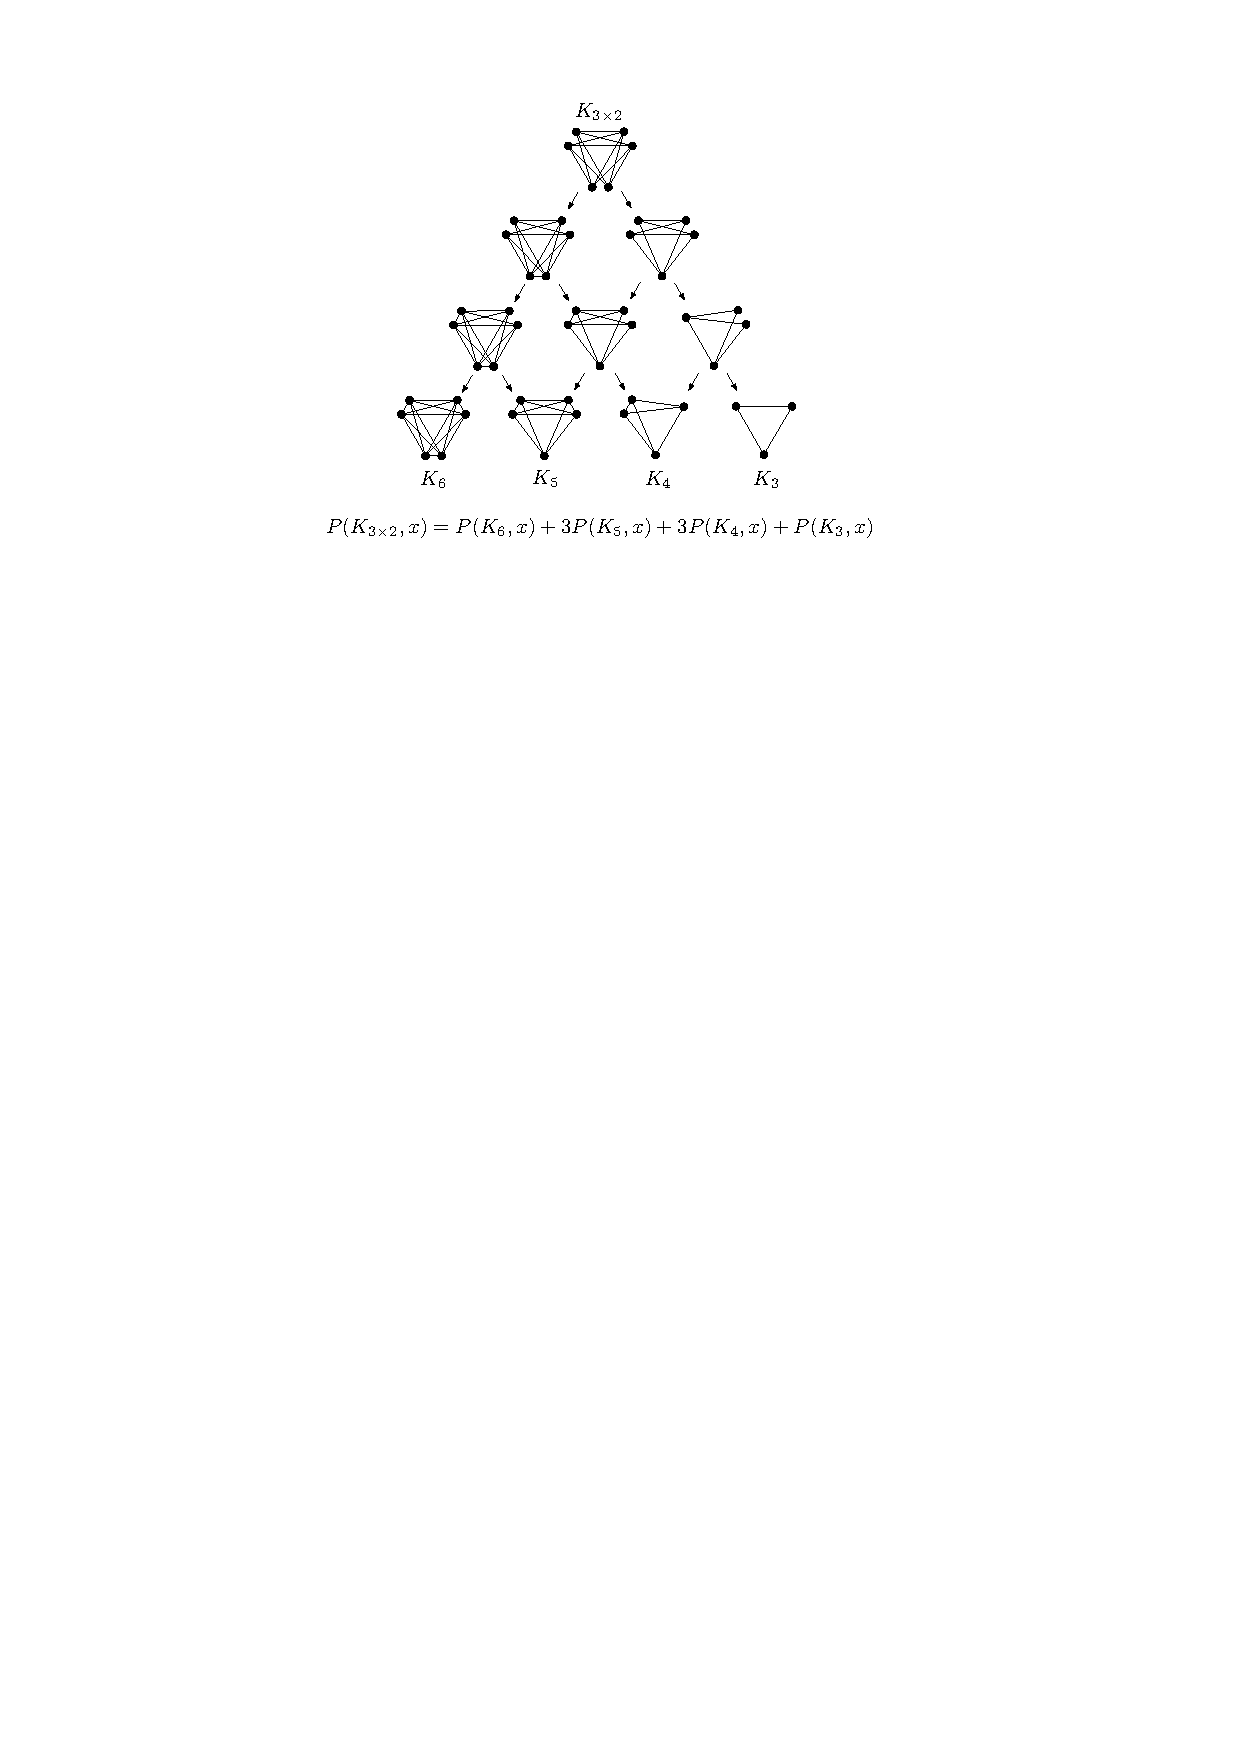
\includegraphics[width=0.8\textwidth]{Resources/Figs/octahedral_pascal_demo.pdf}
    \caption{Demonstration of formula \ref{eqn:chromatic-pascal} on the graph of octahedron}
\end{figure}

\subsection{Chromatic polynomials of Platonic and Archimedean solids}

Because the graphs of Platonic and Archimedean solids are all planar, it follows, that they are also sparse. Thus, it is not practical to use the recursive formula \ref{eqn:chrom_poly_nonedge} which has complete graphs as a base case. We can instead simply reorganize the terms and instead use the following formula:

\begin{equation}\label{eqn:chrompoly-edge}
    P(G,x) = P(G - \{u,v\},x) - P(G \cdot \{u,v\},x)
\end{equation}

where $G - \{u,v\}$ is a graph with edge $\{u,v\}$ deleted and $G \cdot \{u,v\}$ a graph with edge $\{u,v\}$ contracted. 

Using the formula above, we can no longer use the complete graph as a base case. Instead we use the fact that for a tree on $n$ vertices $T_n$, we have $P(T_n,x) = x \cdot (x-1)^{n-1}$. This can be imagined by choosing a root vertex $r$ and directing all edges in $T_n$ towards $r$. Now we can color the vertices sequentially s.t. we start with $r$ and then we color direct children of $r$ and so on. To color $r$, we can use all $x$ colors. For any other vertex $v \neq r$, only the \textit{unique} parent $p$ of $v$ is colored which means that there are $x-1$ free colors for $v$. 

Note that we assume that the graph $G$ that we start with is connected. This assumption comes naturally as we are dealing only with graphs of 3-dimensional solids. We also assume that in the recursive step, we always pick an edge that lies on a cycle. This way, we will never create a disconnected graph. Finding such edge is in practice done using DFS.


An algorithm, that uses formula \ref{eqn:chrompoly-edge} and the assumptions above is implemented in the \textit{SageMath} \cite{sagemath} software under the name \verb|chromatic_polynomial|. The time complexity of this algorithm is exponential in $E(G)$, the number of edges of the graph $G$ on input. By using this algorithm, it is possible to calculate chromatic polynomials of Platonic and Archimedean graphs with at most $48$ edges in the order of minutes.

A more detailed description of how the algorithm is implemented can be found in a technical report by Read \cite{read1987chromatic}.

In the table below we provide examples of chromatic polynomials we computed.

\begin{table}[H]
\centering
\begin{tabular}{lp{0.7\linewidth}}
\toprule
\textbf{Solid} & \textbf{Chromatic polynomial} \\
\midrule
cube & $x^{8} - 12x^{7} + 66x^{6} - 214x^{5} + 441x^{4} - 572x^{3} + 423x^{2} - 133x$ \\
octahedron & $x^{6} - 12x^{5} + 58x^{4} - 137x^{3} + 154x^{2} - 64x$ \\
tetrahedron & $x^{4} - 6x^{3} + 11x^{2} - 6x$ \\
\bottomrule
\end{tabular}
\caption{Chromatic polynomial of selected solids.}
\label{tab:selected-chrom-polys}
\end{table}

